\documentclass[12pt]{article}

\usepackage{lipsum}
\usepackage{fancyhdr}
\usepackage[warn]{mathtext}
\usepackage[T2A]{fontenc}
\usepackage[utf8x]{inputenc}
\usepackage{hyperref}
\usepackage{xcolor}
\usepackage{listings}
\usepackage{xstring}
\usepackage{graphicx}

\definecolor{dkgreen}{rgb}{0,0.6,0}
\definecolor{ltgray}{rgb}{0.5,0.5,0.5}

\makeatletter
\newif\ifcolname
\colnamefalse

\def\keywordcheck{%
\IfStrEq*{\the\lst@token}{select}{\global\colnametrue}{}%
\IfStrEq*{\the\lst@token}{where}{\global\colnametrue}{}%
\IfStrEq*{\the\lst@token}{from}{\global\colnamefalse}{}%
\color{blue}%
}
\def\setidcolor{%
\ifcolname\color{purple}\else\color{black}\fi%
}
\makeatother

\lhead{Рекомендательная система курсов}
\rhead{Страница \thepage}
\renewcommand{\headrulewidth}{0.4pt}
\renewcommand{\footrulewidth}{0.4pt}
\title{Рекомендательная система курсов на графах}
\author{Ахтямов Алексей (mralexeimk@yandex.ru)}
\date{\today}

\lstset{%
    backgroundcolor=\color{white},
    basicstyle=\footnotesize,
    breakatwhitespace=false,
    breaklines=true,
    captionpos=b,
    commentstyle=\color{dkgreen},
    deletekeywords={...},
    escapeinside={\%*}{*)},
    extendedchars=true,
    frame=single,
    keepspaces=true,
    language=SQL,
    otherkeywords={is},
    morekeywords={*,modify,MODIFY,...},
    keywordstyle=\keywordcheck,
    identifierstyle=\setidcolor,
    numbers=left,
    numbersep=15pt,
    numberstyle=\tiny,
    rulecolor=\color{ltgray},
    showspaces=false,
    showstringspaces=false, 
    showtabs=false,
    stepnumber=1,
    tabsize=4,
    title=\lstname
}

\begin{document}
\maketitle

\section*{Введение}
В текущем документе описывается построение эффективной конфигурации базы данных PostgreSQL с таблицами курсов и тэгов, создание рекомендательной системы курсов, основанной на графах и извлечение тэгов из пользовательского ввода (в поле поиска курсов) с помощью расстояние Левенштейна. \newline
Реализация на Python представлена тут \href{https://github.com/Yedom/RecomendationSystem}{\color{blue}GitHub}.
\section*{Структура базы данных}
База данных будет содержать 2 таблицы (\textbf{'coursers'} и \textbf{'tags'}) \newline

\noindent \textbf{Coursers:} \newline
Тип: \textit{динамически обновляемая} \newline
Пример создания \textbf{'coursers'} таблицы с помощью SQL запроса (нам важны только столбцы \textbf{id}, \textbf{title} (название курса) и \textbf{tags} (тэги)): \newline

\begin{lstlisting}[language=sql]
CREATE TABLE coursers (
	id SERIAL PRIMARY KEY,
	title VARCHAR (255) NOT NULL,
	author VARCHAR (255) NOT NULL,
	views INTEGER NOT NULL,
	likes INTEGER NOT NULL,
	tags TEXT NOT NULL)
\end{lstlisting}

\noindent Таблица будет содержать список добавленных курсов. \newline
Столбец \textbf{tags} содержит набор строк (тэгов), разделенных специальным символом (в нашей реализации это символ \textbf{'@'}). \newline

\noindent \textbf{Tags:} \newline
Тип: \textit{периодически обновляемая} \newline
Создание \textbf{'tags'} таблицы с помощью SQL запроса: \newline
Заполнение происходит периодически из таблицы \textbf{'coursers'} \newline

\begin{lstlisting}[language=sql]
CREATE TABLE tags (
	id SERIAL PRIMARY KEY,
	tag VARCHAR(255) UNIQUE NOT NULL,
	coursers_count INTEGER NOT NULL,
	related_tags TEXT)
\end{lstlisting}

\noindent Таблица будет хранить список всех тэгов. \newline
Столбец \textbf{coursers\_count} хранит число курсов, использующих тэг. \newline
Столбец \textbf{related\_tags} хранит индексы тэгов, связанных с текущим. \newline
Для ускорения обновления таблицы и ограничения числа смежных вершин в графе введем ограничение на количество тэгов, связанных с текущим. Обозначим это ограничение сверху как \underline{\textbf{maxRelatedTags}}. При периодическом обновлении таблицы в столбец \textbf{related\_tags} войдут индексы тех тэгов, \textbf{coursers\_count} которых в таблице наибольший. \newline

\section*{Построение графа}
\href{https://getfile.dokpub.com/yandex/get/https://disk.yandex.ru/d/yRuwHZWdXBIIaA}{\color{blue}Визуальный пример} графа с тэгами и курсами. \newline
Обозначим число курсов как \textbf{coursersCount}, а число тэгов как \textbf{tagsCount}. \newline
Граф - множество вершин, соединенных между собой каким-то образом. Ориентированный граф - граф, с ориентированным соединением между вершинами. \newline \newline
Вершинами нашего графа будут все тэги и все курсы ($tagsCount + coursersCount$). Каждая вершина имеет максимум \textbf{maxRelatedTags} выходящих из нее ребер, ведущих к вершинам-тэгам и максимум \textbf{coursersCount} выходящих ребер, ведущих к вершинам-курсам. \newline
\textit{В худшем случае}, \textbf{когда каждый тэг есть в каждом курсе}, используемая для хранения графа память равна $O(V+E) = O((tagsCount + coursersCount) + (tagsCount + coursersCount)*(maxRelatedTags + coursersCount))$ \newline

\noindent Перебирая значения двух переменных при $maxRelatedTags = 5$ получаем: \newline
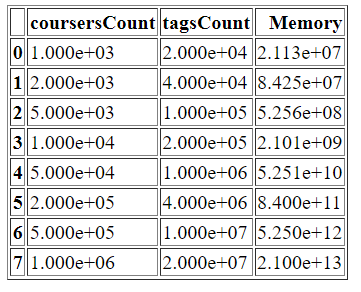
\includegraphics[scale=1.2]{images/memory.png} \newline
Для хранения графа с миллионом курсов и $20$-ти миллионами тэгов требуемая память составляет $\sim 2 \cdot 10^{13}$ бит (40000 ГБ). \newline

\noindent Пусть \textbf{averageCoursersOnTag} - среднее число курсов, содержащих определенный тэг. \newline
\textit{В среднем случае}, требуемая память составляет $O((tagsCount + coursersCount) + (tagsCount + coursersCount)*(maxRelatedTags + averageCoursersOnTag))$ \newline
Перебирая значения двух переменных при $maxRelatedTags = 5$ получаем: \newline
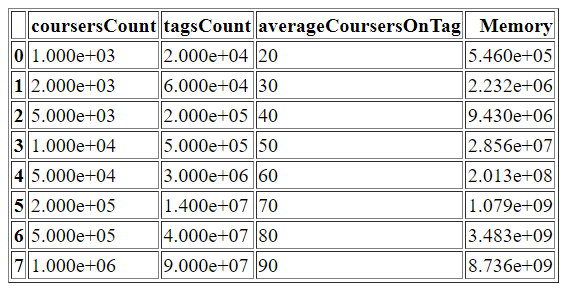
\includegraphics[scale=1.2]{images/memoryAverage.png} \newline
Для хранения графа с миллионом курсов и $90$-та миллионами тэгов требуемая память составляет $\sim 9 \cdot 10^{9}$ бит (4 ГБ). \newline

Инициализация графа происходит периодически после обновления таблицы \textbf{'tags'}.

\section*{Обработка пользовательского ввода}
Для поиска тэгов в пользовательской строке разобьем строку на слова (разделенные пробелом) переберем все размещения из количества слов по $i$, $\forall i \leq maxWordsInTag$ (\textbf{maxWordsInTag} - максимальное число слов в тэге, в нашей реализации оно равно $3$). \newline
В каждом размещении объеденим слова в строку и с помощью бинарного поиска найдем окрестность похожих на нее тэгов. Выберим из них тот, расстояние по Левенштейну до которого минимально и, если это расстояние меньше какой-то верхней границы - берем этот тэг для дальнейшей рекомендации по нему. \newline
Расстояние Левенштейна - минимальное число операций (удаление, вставка и замена символа), необходимых для превращения одной строки в другую. Чем оно меньше - тем более похожи строки. В нашей реализации, для избежания эквивалентности коротких тэгов, операция замены стоит в 2 раза больше других операций. \newline
После обработки мы получим список тэгов, по которым мы будем рекомендовать пользователю курсы. \newline

\section*{Рекомендация курсов}
После получения списка тэгов, добавим в этот список семантически частные тэги. \newline
В нашем графе, если вершина-тэг A идет в вершину-тэг B означает, что B - более высокая абстракция над A или, по-другому, A - частный случай B. \newline
Для добавления новых тэгов, переберем все смежные вершины-тэги в графе у списка тэгов и добавим в список. Проделаем эту операцию столько раз, какую глубину мы указали в конфигурации. \newline
В итоге, мы имеем список тэгов и информацию о том, на какой глубине получен этот тэг. Переберем все эти тэги в графе и найдем все смежные вершины-курсы и добавим в нашу рекомендацию. В зависимости от глубины, ключевых слов в названии курса или рейтинга сформируем и отсортируем список рекомендуемых курсов.
\end{document}